\documentclass[10pt]{article}
\usepackage{amsmath,textcomp,amssymb,geometry,graphicx,enumerate,tikz,algorithm,algpseudocode,pifont}
\usetikzlibrary{calc}
\usetikzlibrary{datavisualization}
\usetikzlibrary{datavisualization.formats.functions}


\textheight=9in
\textwidth=7in
\topmargin=-.75in
\oddsidemargin=-0.25in
\evensidemargin=-0.25in

\usepackage{listings}
\lstnewenvironment{codeblock}
    {\lstset{language=Python,
      showspaces=false,
      showtabs=false,
      breaklines=true,
      mathescape=true,
      showstringspaces=false,
      breakatwhitespace=true,
      commentstyle=\textit,
      keywordstyle=\textbf,
      basicstyle=\ttfamily,
      escapechar=`,
      moredelim={**[is][{\color{RoyalBlue}}]{\^^M\\beginsol}{\^^M\\endsol}},
      moredelim={[is][{\color{RoyalBlue}}]{\^^M\\beginexp}{\^^M\\endexp}},
    }}
    {}

\begin{document}
\section*{02/08/2016}
	\subsection*{Decision Theory}
	\
	\begin{itemize}
		\item Multiple samples with different classes could lie on the same point.
		\item We want a probabilistic classifier.
		\item Suppose 10\% of the population has cancer; 90\% doesn't. We have a probability distribution for calorie intake, $P(X|Y)$:
		\begin{center}
			\begin{tabular}{| c | c | c | c |}
				\hline
 				Calories(X) & $< 1200$ & $1200 - 1600$ & $> 1600$\\
 				\hline
 				Cancer (Y=1) & 20\% & 50\% & 30\%\\
 				\hline
 				no cancer (Y=-1) & 1\% & 10\% & 89\%\\
 				\hline
			\end{tabular}
		\end{center}
	
		\item Recall: $P(X) = P(X|Y=1)P(Y=1) + P(X|Y=-1)P(Y=-1)$
		\item $P(1200 \leq X \leq 1600) = 0.5\cdot 0.1 + 0.1\cdot 0.9 = 0.14$
		\item You meet guy eating $x = 1400$ cals/day. Guess whether he has cancer?
		\item \textbf{Bayes' Theorem}:
			\begin{align*}
				P(A=a|B) &= \frac{P(B|A=a)P(A=a)}{P(B)}\\
				P(Y=1|X=1400) &= \frac{P(X=1400|Y=1)P(Y=1)}{P(X=1400)} = \frac{0.05}{0.14} \\
				P(Y=-1|X=1400) &= \frac{P(X=1400|Y=-1)P(Y=-1)}{P(X=1400)} \frac{0.09}{0.14} \\
				P(Y=1|X=1400) &= \frac{5}{14} \approx 36\% \ \text{probability guy with 1400 cal/day has cancer}\\
			\end{align*}
		\item A \underline{loss function} $L(z, y)$ specifies badness if true class is $y$; classifier prediction is $z$.
			\[
 				L(z, y) = \left\{\def\arraystretch{1.2}%
 					\begin{array}{@{}c@{\quad}l@{}}
    					1 & \text{if $z=1, y=-1$}\\
   						5 & \text{if $z=-1, y=1$}\\
   						0 & \text{otherwise}\\
						\end{array}\right.
			\]
		\item Definitions: 
			\begin{itemize}
				\item loss function above is \underline{asymmetrical}
				\item The \underline{0-1 loss function} is 1 for incorrect predictions, 0 for correct.
			\end{itemize}
		\item Let $r: \mathbb{R}^{d} \rightarrow \pm 1$ be a \underline{decision rule}, aka \underline{classifier}: a function that maps a feature vector $x$ to 1 ("in class") or -1 ("not in class").
		\item The \underline{risk} for $r$ is the expected loss over all values of $x,y$:
			\begin{align*}
				R(r) &= E[L(r(X), Y)]\\
					&= \sum_{x} (L(r(x), 1)P(Y=1|X=x) + L(r(x), -1)P(Y=-1|X=x))P(x)\\
					&= \sum_{x} (L(r(x), 1)\frac{P(X=x|Y=1)(P(Y=1)}{P(x)} 
							+ L(r(x), 1)\frac{P(X=x|Y=-1)(P(Y=-1)}{P(x)})P(x)\\
					&= P(Y=1)\sum_{x} L(r(x), 1)P(X=x|Y=1) +
						P(Y=-1)\sum_{x} L(r(x), -1)P(X=x|Y=-1)\\
			\end{align*}
		\item The \underline{Bayes optimal decision rule} aka \underline{Bayes classifier} is the $r$ that minimizes $R(r)$; call it $r^{*}$. Assuming $L(z, y) = 0$ for $z=y$:
			\[
 				r^{*}(x) = \left\{\def\arraystretch{1.2}%
 					\begin{array}{@{}c@{\quad}l@{}}
    					1 & \text{if $L(-1,1)P(Y=1|X=x) > L(1,-1)P(Y=-1|X=x$)}\\
   						-1 & \text{otherwise}\\
						\end{array}\right.
			\]
		\item In cancer example, $r^{*} = 1$ for all intakes $\leq 1600$; $r^{*} = -1$ for intakes $\geq 1600$, then the \underline{Bayes risk}, aka \underline{optimal risk} is:
		\begin{align*}
			R(r^{*}) = 0.1(5\cdot 0.3) + 0.9(1 \cdot 0.01 + 1 \cdot 0.1) = 0.249\\
		\end{align*}
		\item Suppose $X$ has a continuous probability density function (PDF):
		\item Review:
			\begin{itemize}
				\item probability that random variable
				$X \in [x_{1}, x_{2}] = \int_{x_{1}}^{x_{1}} P(x) dx$\\
				\item area under whole curve $\int_{-\infty}^{\infty} P(x) dx = 1$\\
				\item \underline{expected} value of $f(x): E[f(x)] = \int_{-\infty}^{\infty} f(x)P(x) dx$\\
				\item \underline{mean} $\mu = E[x] = \int_{-\infty}^{\infty} xP(x) dx$\\
				\item \underline{variance} 
					$\sigma^{2} = E[(X-\mu)^{2}] = E[X^{2}] - \mu^{2}$\\
					\begin{center}
						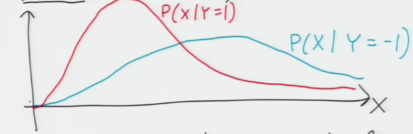
\includegraphics[scale=0.5]{../images/gaus}
					\end{center}
				\item Suppose $P(Y=1) = \frac{1}{3}$, $P(Y=-1) = \frac{2}{3}$.
					\begin{center}
						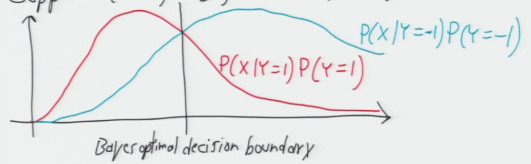
\includegraphics[scale=0.5]{../images/othrgaus}
					\end{center}
			\end{itemize}
		\item Define \underline{risk} as before, replace summations with integrals.
			\begin{align*}
				R(r) &= E[L(r(X), Y)]\\
					&= \int_{x} (L(r(x), 1)P(Y=1|X=x) + L(r(x), -1)P(Y=-1|	X=x))P(x)dx\\
					&= P(Y=1)\int_{x} L(r(x), 1)P(X=x|Y=1)dx +
					P(Y=-1)\int_{x} L(r(x), -1)P(X=x|Y=-1)dx\\
			\end{align*}
		\item If $L$ is 0-1 loss, $R(r) = P(r(x)) \ \text{is wrong}$\\
		\item For Bayes decision rule, Bayes Risk is the area under the minimum of the functions above. Assuming $L(z,y) = 0$ for $x=y$:
			\begin{align*}
			R(r^{*}) = \int min_{y \pm 1} L(-y, y)P(X=x|Y=y)P(Y=y)dx\\
			\end{align*}
		\item \underline{Bayes optimal decision boundary}: $\{x: P(Y=1|X=x) = 0.5\}$.
			\begin{center}
				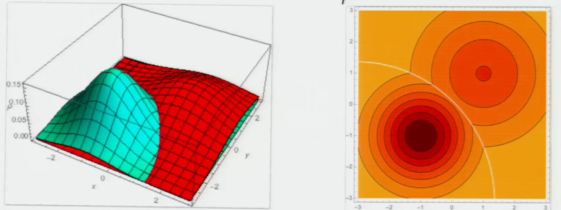
\includegraphics[scale=0.5]{../images/cancergaus}
			\end{center}
	\end{itemize}
	
	\subsection*{3 Ways to Build Classifiers}
	\
		\begin{enumerate}
			\item Generative models (e.g. LDA)
				\begin{itemize}
					\item Assume samples come from probability distributions, different for each class.
					\item Guess form of distributions.
					\item For each class C, fit distribution parameters for class C samples, giving $P(X|Y=C)$.
					\item For each C, estimate $P(Y=C)$.
					\item Bayes' Theorem gives $P(Y|X)$.
					\item If 0-1 loss, pick class C that maximizes $P(Y=C|X=x)$. Equivalently, maximizes $P(X=x|Y=C)P(Y=C)$.
				\end{itemize}
			\item Discriminative models (e.g. logistic regression)
				\begin{itemize}
					\item Model $P(Y|X)$ directly 
				\end{itemize}
			\item Find decision boundary (e.g. SVM).
				\begin{itemize}
					\item Model $r(x)$ directly (no posterior).
				\end{itemize}
		\end{enumerate}
		
		\begin{itemize}
			\item Advantages of (1, 2): $P(Y|X)$ tells you probability your guess is wrong.
			\item Advantage of (1): you can diagnose outliers: $P(x)$ is very small.
			\item Disadvantages of (1): often hard to estimate distribution accurately; real distributions rarely match standard ones.
		\end{itemize}
\end{document}
